\section{Performance}
The performance and resource utilization of the game has been tested using Visual Studio's performance profiler\footnote{\url{https://learn.microsoft.com/en-us/visualstudio/profiling/?view=vs-2022}}.
The analysis was focused on three aspects:
\begin{enumerate}
    \item File I/O,
    \item CPU usage,
    \item memory usage.
\end{enumerate}
The data was collected on a machine running on x64-based Windows 11 with Intel(R) Core(TM) i7-9750H CPU, 32 GB of RAM, and NVIDIA GeForce GTX 1650 GPU.
During the first minute of the data collection, the player was running constantly, approximately in one direction, while modifying the terrain at the same time.
Starting at the 1-minute mark, the player turned around and started running in the opposite direction, still modifying the terrain, and also shooting at the bots from time to time.
The results of the profiling are shown in \autoref{fig:diag-session}.
\begin{figure}[h]
    \centering
    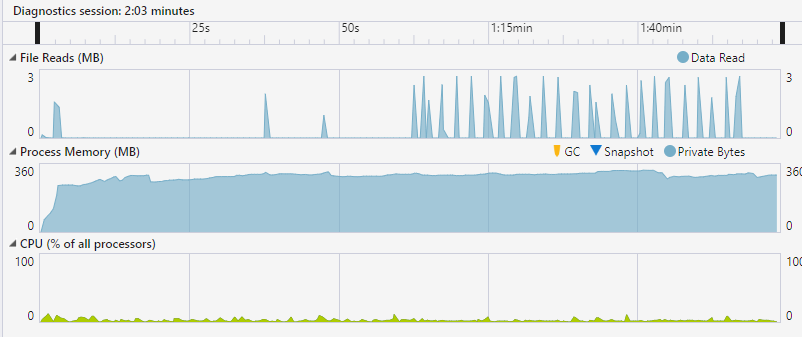
\includegraphics[width=1\textwidth]{chapters/results/sections/performance/resources/diag-session.png}
    \caption{Resource utilization of the game}
    \label{fig:diag-session}
\end{figure}

The "File Reads" graph shows the amount of data read in MB.
The initial spike in the file reads corresponds to the game reading the shader files and PNG files with textures.
It can be seen that starting at the 1-minute mark, there are frequent file reads.
This is because the chunks that were generated (and subsequently removed from the game and saved) during the initial run in one direction are now being revisited by the player and read from the disk.

The "Process Memory" graph shows that the memory usage remains approximately constant at around 350 MB.

The "CPU" graph shows that the CPU utilization peaks at around 10\%.

The total amount of disk space required to store the game saves for this session was 100 MB.